%%
%TC:ignore
%\small
\subsection*{Model} \label{sec:model}

We modeled microbial abundances over time along the lines of Blumm \textit{et al.}\cite{ranking}. The dynamics of taxon relative abundances was described by the Langevin equation:
\begin{linenomath}
\begin{equation*}
\dot{x_i} = F_i \cdot x_i^\alpha + V \cdot x_i^\beta \xi_i(t) - \phi(t) \cdot x_i,
\end{equation*}
\end{linenomath}
where $F_i$ captured the fitness of the taxon $i$, $V$ corresponded to the noise amplitude and $\xi_i$(t) was a Gaussian random noise with zero mean  $<\xi_i(t)> = 0$, and variance which was uncorrelated over time, $<\xi_i(t) \xi_i(t')> = \delta(t'-t)$. The function $\phi(t)$ ensured the normalization at all times, $\sum x_i(t) = 1$, and corresponded to $\phi(t) = \sum F_i x_i^\alpha + \sum V x_i^\beta \xi_i(t)$.
The temporal evolution of the probability that taxon $i$ had a relative abundance $x_i(t)$, $P(x_i,t)$, was determined by the Fokker-Planck equation:
\begin{linenomath}
\begin{equation*}
\frac{\partial P}{\partial t} = - \frac{\partial}{\partial x_i}  [(F_i \cdot x_i^\alpha - \phi(t) \cdot x_i ) \cdot P]+ \frac{1}{2} \frac{\partial^2}{\partial x_i^2} (V^2 \cdot x_i^{2\beta}\cdot P).
\end{equation*}
\end{linenomath}
The microbiota evolved towards a steady state with a time-independent probability dependent on the values of $\alpha$, $\beta$, $F_i$ and $V$. For $\alpha<1$ (otherwise, systems are always unstable), the steady state probability was localized in a region around a preferred value or broadly distributed over a wide range, depending on whether the fitness $F_i$ dominated or was overwhelmed by the noise amplitude $V$. The steady-state solution of the Fokker--Planck equation was given by:
\begin{eqnarray*}
P_0 (x_i) &=& C_{ne}(\alpha,\beta,F_i,V)  \cdot x_i^{-2\beta}  \cdot \exp\Big[\frac{2F_i}{V^2}\frac{x_i^{1+\alpha-2\beta}}{1+\alpha-2\beta}-\frac{\phi_0}{V^2}\frac{x_i^{2-2\beta}}{1-\beta}\Big] \quad \textrm{if} \quad  2\beta \ne 1+\alpha, \\
P_0 (x_i) &=& C_e(\alpha,\beta,F_i,V)  \cdot x_i^{\frac{2F_i}{V^2} -2\beta}  \cdot \exp\Big[\frac{\phi_0}{V^2}\frac{x_i^{2-2\beta}}{1-\beta}\Big] \quad \textrm{if} \quad  2\beta = 1+\alpha,
\end{eqnarray*}
where $\phi_0 = (\sum_i F_i^{1/(1-\alpha)})^{1-\alpha}$ and $C_{ne}$ and $C_{e}$ were integrals that were solved numerically for the parameters of interest. The ordered phase occurred when the solution had a maximum in the physical interval ($0<x_i<1$). For a larger V, the transition to a disordered phase happened when the maximum shifted to the unphysical region $x_i<0$, which sets the phase transition region $V(\alpha,\beta,F_i)$. The phase transition region was calculated analytically in specific cases:
\begin{eqnarray*}
F_i^2 &=& 4 \beta \phi_0 V^2\quad \textrm{if} \quad  \beta = \alpha \neq 1,\\
F_i &=& \beta V^2\quad \textrm{if} \quad  2\beta = 1+\alpha,
\notag
\end{eqnarray*}
where the first case, simplified to $F = 3 V^2$ if $\beta = 0.75$ and the fitness of this taxon dominated in $\phi_0$. 
In many physical systems (Brownian motion is the classic example \cite{Einstein}), the two terms of the Langevin's equation are related.  The \emph{Fluctuation Dissipation Theorem} states out a general relationship between the response to an external disturbance and the internal fluctuations of the system\cite{FD}. The theorem can be used as the basic formula to derive the fitness from the analysis of fluctuations 
of the microbiota, assuming that it is in equilibrium (the ordered phase).  

%%
\subsection*{Standardization} \label{sec:stan}
In order to properly show all the studies under common axes, we decided to standardize the Taylor parameters using the group of healthy individuals for every single study independently. With this approach, all the studies can be visualized in a shared plot with units of Taylor--parameter standard--deviation on their axes.

For a Taylor's parameter, e.g. $V$, the estimate of the mean ($\widehat{V}$) for the healthy subpopulation, composed of $h$ individuals, is:
\begin{linenomath}
$$\widehat{V} = \frac{1}{W_1}\sum_{i=1}^h V_i \omega_i=\sum_{i=1}^h V_i \omega_i$$
\end{linenomath}
as $W_1=\sum_i^h \omega_i=1$, since $\omega_i$ are normalized weights calculated as:
\begin{linenomath}
$$\omega_i = \frac{\frac{1}{\sigma^2_{V_i}}}{\sum_i^h\frac{1}{\sigma^2_{V_i}}}$$
\end{linenomath}
$\sigma_{V_i}$ being the estimation of the uncertainty in $V_i$ obtained together with $V_i$ from the X-weighted power-law fit described in Section \ref{sec:X-w}, for healthy individuals.

Likewise, the estimation of the standard deviation for the healthy population ($\widehat{\sigma}_V$) is:
\begin{linenomath}
$$\widehat{\sigma}_V = \sqrt{\frac{1}{W_1-\frac{W_2}{W_1}}\sum_{i=1}^h\left[\omega_i\left(V_i-\hat{V}\right)^2\right]}$$
\end{linenomath}
with $W_2=\sum_i^h \omega_i^2$, which finally yields to:
\begin{linenomath}
$$\widehat{\sigma}_V = \sqrt{\frac{1}{1-\sum_i^h \omega_i^2}\sum_{i=1}^h\left[\omega_i\left(V_i-\hat{V}\right)^2\right]}$$
\end{linenomath}

%%
\subsection*{Selection and Methods}

The bacteria and archaea taxonomic assignations were obtained by analyzing 16S rRNA sequences, which were clustered into operational taxonomic units (OTUs) sharing 97\% of their sequence identity using QIIME \cite{QIIME}. Shotgun metagenomic sequencing (SMS) data\cite{kwashiorkor} were analyzed and assigned at strain level by the Livermore Metagenomic Analysis Toolkit (LMAT)\cite{LMAT}, according to their default quality threshold. Genus, with the best balance between error assignment and number of taxa, was chosen as our reference taxonomic level. We verified that our conclusions were not significantly affected by selecting family or species as the reference taxonomic level (see Supplementary Figure S\ref{supfig:taxlev1}).

%%
\subsubsection*{Sample selection}
We chose studies about relevant pathologies containing metagenomic sequencing time data series of bacterial populations from humans in different healthy and non-healthy states. Only those individuals who had three or more time points of data available in databases were selected. The study by Caporaso \textit{et al.} study \cite{moving} was selected as it featured two healthy individuals measured over a very long timespan, with almost daily sampling. The study of Faith \textit{et al.} \cite{LEA} was selected given the BMI differences between subjects. Moreover, some of them followed diets which could be treated as system perturbations. Only those individuals who had normal or overweight BMI were considered as healthy. The study by Smith \textit{et al.} \cite{kwashiorkor} was selected for both the age of the patients and the rare disease. We only worked with the discordant twins, and considered those who were not affected by kwashiorkor in each pair of patients as being healthy. The study by David \textit{et al.} \cite{diet} was selected for its differential diets. The healthy part was considered to be the first time samples of each individual before the diet, while the rest of the time points were considered as perturbations. Dethlefsen and Relman's work \cite{antibiotic} was selected due to the interesting treatment of two antibiotic intakes by three different subjects of the same antibiotic. The healthy part was considered to be only those times before any antibiotic treatment, and the time of antibiotic intakes and the period after that as perturbations. The work by David \textit{et al.} \cite{hostlife} was selected due to the comprehensive longitudinal data that it provides plus its complete metadata and the interesting events that happened to both subjects (an infection and a trip abroad). The healthy part was taken from time points before or after each event. Finally, we also considered a study from our group carried out by Durban \textit{et al.} \cite{IBS} in which the healthy subjects were considered as those who did not suffer from irritable bowel syndrome, while the patients who had this disease were taken as perturbations. 

The metadata for each study is provided in Supplementary Tables S\ref{tab:diet} to S\ref{tab:LEA}. They all used 16S rRNA gene sequencing, except for the study of the discordant kwashiorkor twins\cite{kwashiorkor}, in which both SMS and 16S rRNA data were used. In the latter case, we chose to work with SMS data to show that our method was valid, regardless of the source of taxonomic information. Each of the datasets was treated as follows:

%%
\subsubsection*{16rRNA sequences processing}
Reads from the selected studies were first quality filtered using the FastX toolkit\cite{FASTX}, allowing only those reads which had more than a quality score of over 25 in 75\% of the complete sequence. 16S rRNA reads were then clustered at a 97\% nucleotide sequence identity (97\% ID) into operational taxonomic units (OTUs), using the QIIME software package\cite{QIIME} (version 1.8). We followed an open reference OTU picking workflow in all cases. The clustering method used was UCLUST, and the OTUs were matched against the Silva database\cite{SILVA} (version 111, July 2012) and were assigned to a taxonomy with a UCLUST-based consensus taxonomy assigner. The parameters used in this step were: similarity 0.97, prefilter percent id 0.6, maximum accepts 20, maximum rejects 500. 

%%
\subsubsection*{Metagenomic sequences processing}
Shotgun metagenomic sequences were analyzed with LMAT (Livermore Metagenomics Analysis Toolkit) software package\cite{LMAT} (version 1.2.4, with Feb'15 release of the LMAT-Grand database). LMAT was run using a Bull shared-memory node belonging to the team?s HPC (high performance computing) cluster. It was equipped with 32 cores (64 threads available using Intel Hyper-Threading Technology) as it has two Haswell-based Xeons (22 nm technology), the E5-2698v3@2.3 GHz, sharing half a tebibyte of DRAM memory. This node is also provided with a PCIe SSD card as NVRAM, the Micron P420m HHHL, with 1.4 TB, and 750000 reading IOPS, 4 KB, achieving 3.3 GB/s. The computing node was supplied with a RAID-0 (striping) scratch disk area. We used the ``Grand'' database\cite{LMAT2}, released in Feb'15, provided by the LMAT team, where ``Grand'' refers to a huge database that contains k-mers from all the viral, prokaryote, fungal and protist genomes present in the NCBI database, plus the Human reference genome (hg19), plus GenBank Human, plus the 1000 Human Genomes Project (HGP) (this represents about 31.75 billion k-mers occupying 457.62 GB)\cite{LMAT2}. Before any calculations were made, the entire database was loaded into the NVRAM. With this configuration, the observed LMAT sustained sequence classification rate was $20\unclassrate$. Finally, it is worth mentioning that a complete set of Python scripts  was developed as back-end and front-end of the LMAT pipeline in order to manage the added complexity of time series analysis (\href{https://github.com/DLSteam/MAUS_scripts}{[https://github.com/DLSteam/MAUS\_scripts]}). 

%%
\subsubsection*{Taxa level robustness}
We selected genus as the taxonomic level for the subsequent steps of our work. In order to ensure that there were no crucial differences between adjacent taxonomic levels which could still be of relevance after standardization (see the last subsection of Material and Methods), we tested two different data sets. In the former, the antibiotics study\cite{antibiotic} with 16S data, we tested the differences between genus and family levels. The latter dataset tested was the kwashiorkor discordant twins study\cite{kwashiorkor} for both genus and species taxonomic levels. The Supplementary Figures S\ref{supfig:taxlev1} (overview) and S\ref{supfig:taxlev2} (detail) plot the comparison between studies (and so, 16S and SMS) and between adjacent taxonomic levels.

%TC:endignore
\begin{supfig} 
  %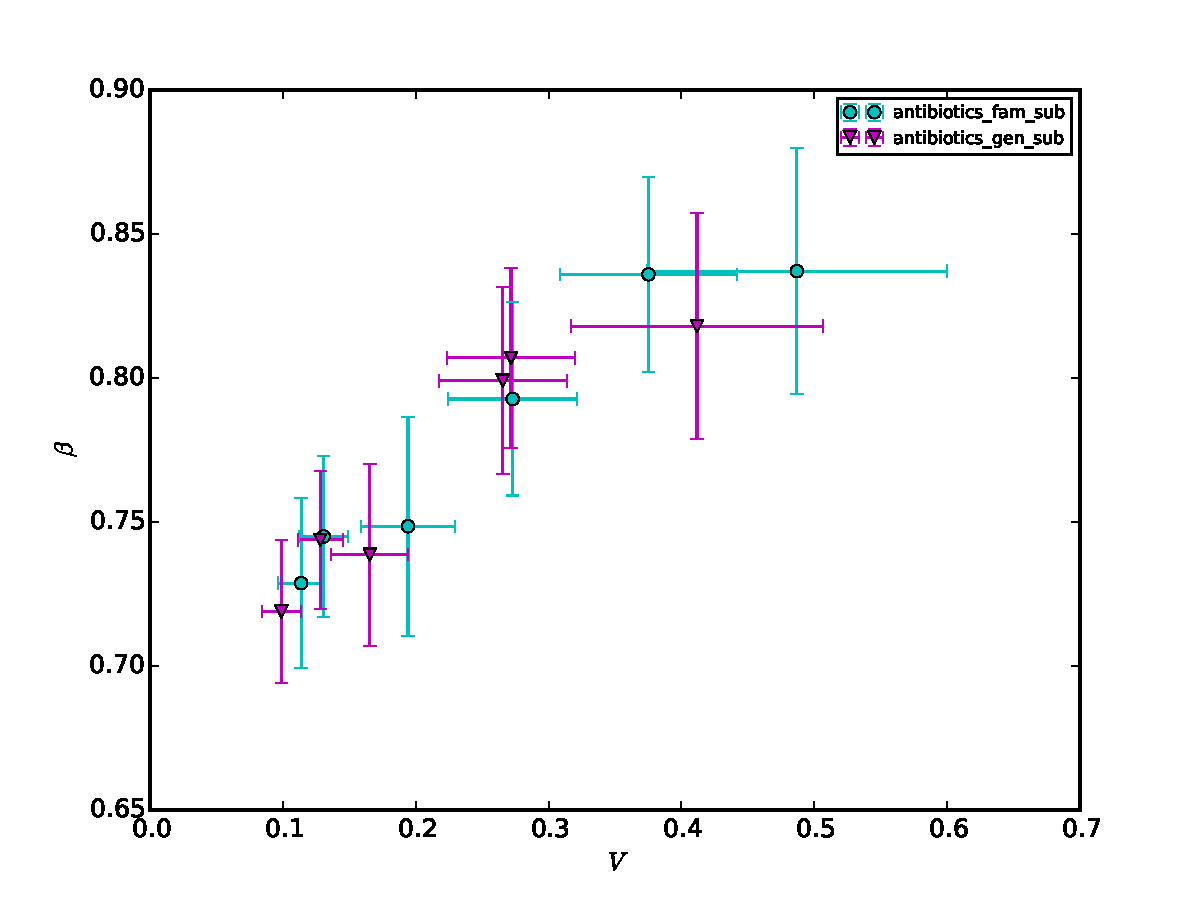
\includegraphics[width=0.5\textwidth]{results/taxalevel/sum_raw_16S.pdf}
  %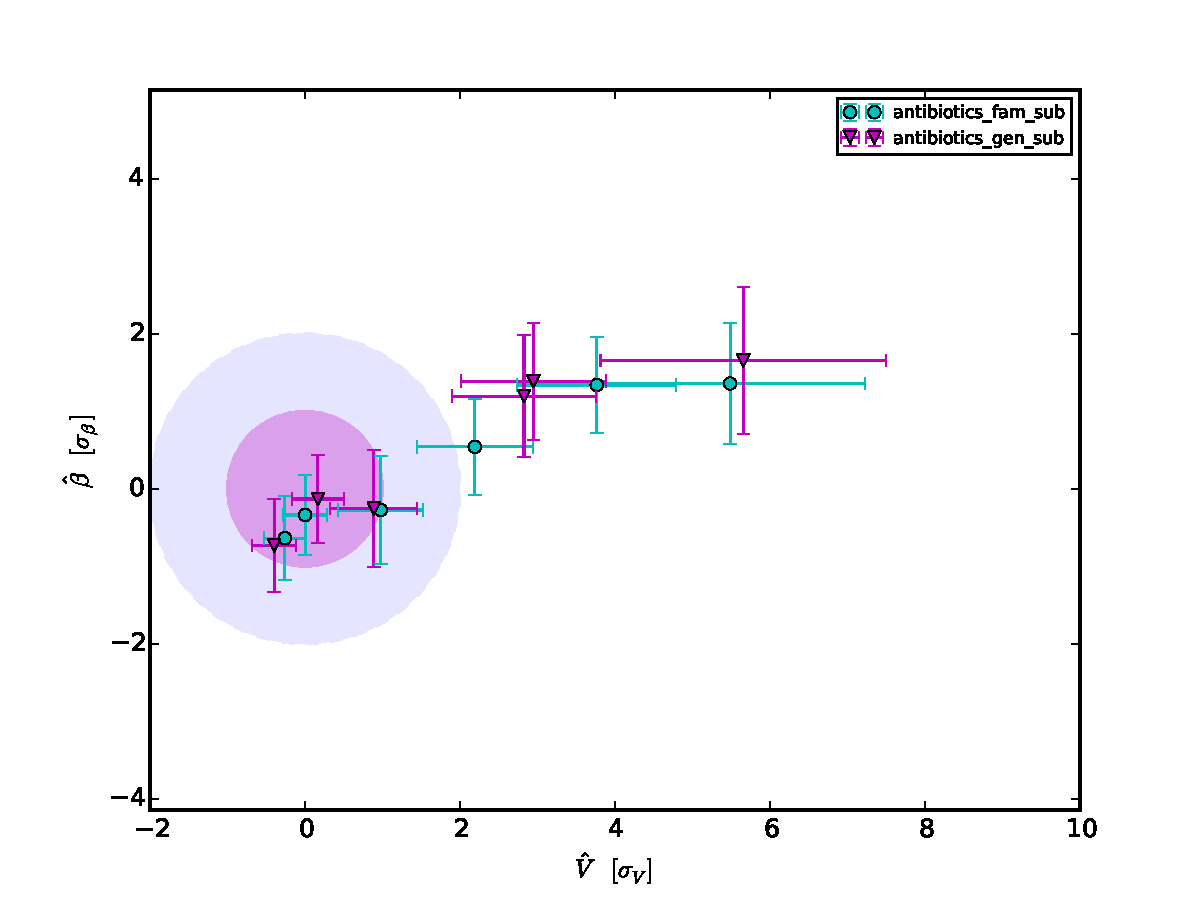
\includegraphics[width=0.5\textwidth]{results/taxalevel/sum_sta_16S.pdf}
  %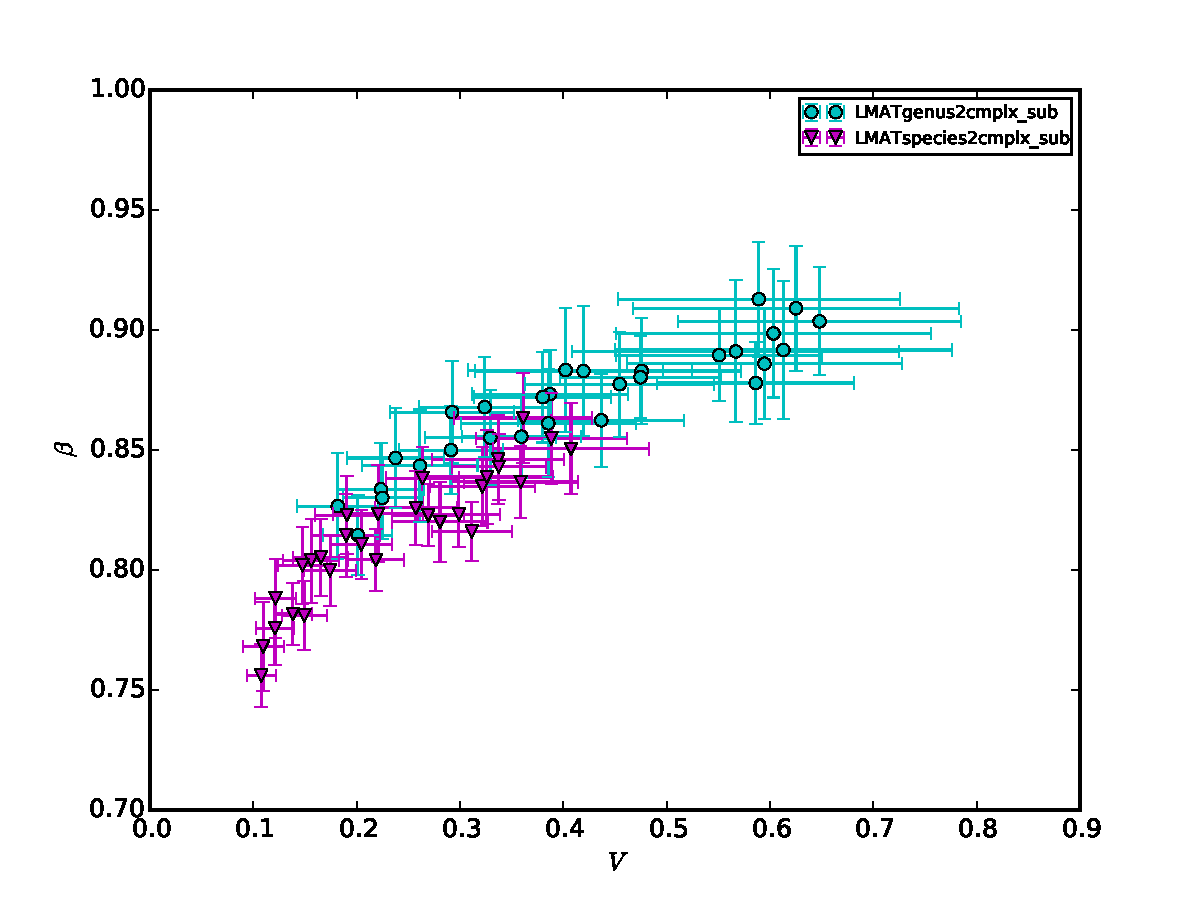
\includegraphics[width=0.5\textwidth]{results/taxalevel/sum_raw_SMS.pdf} 
  %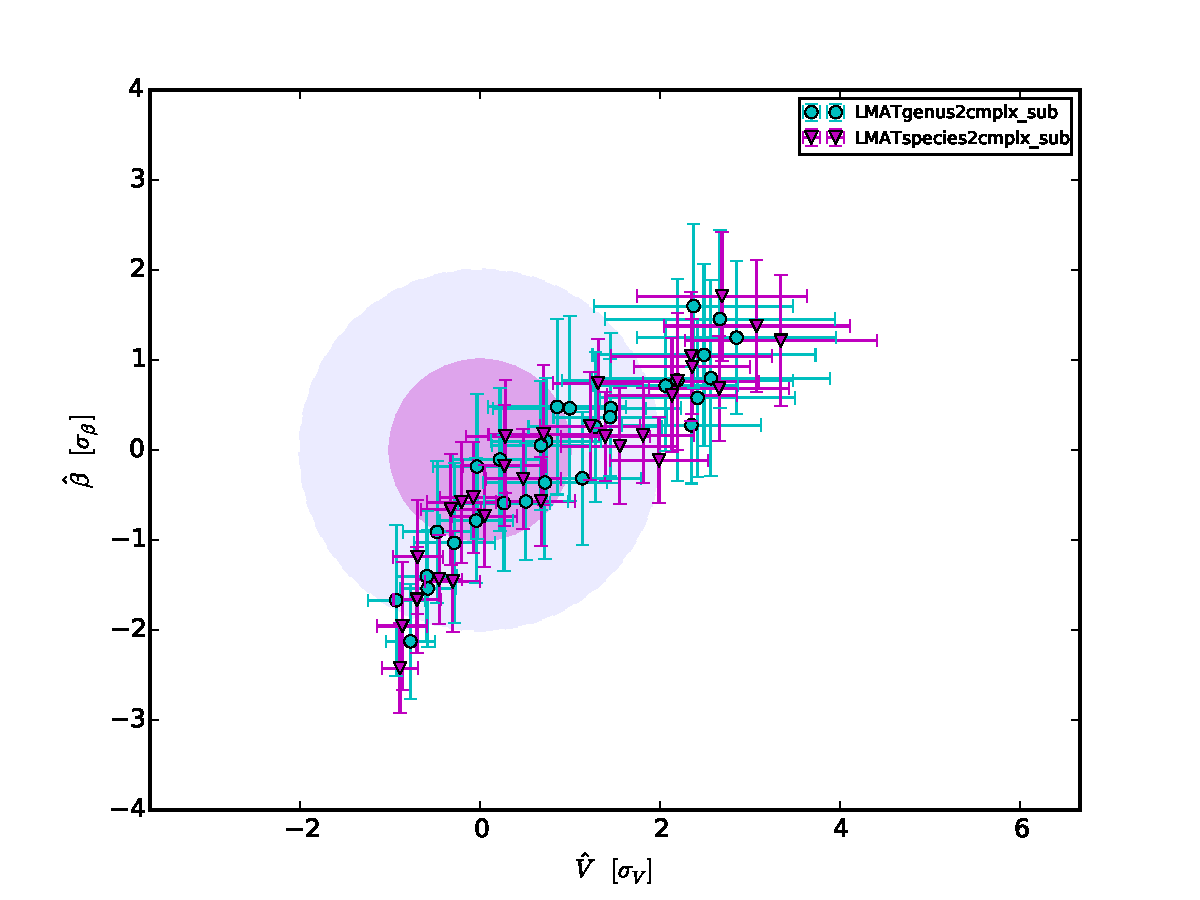
\includegraphics[width=0.5\textwidth]{results/taxalevel/sum_sta_SMS.pdf}
  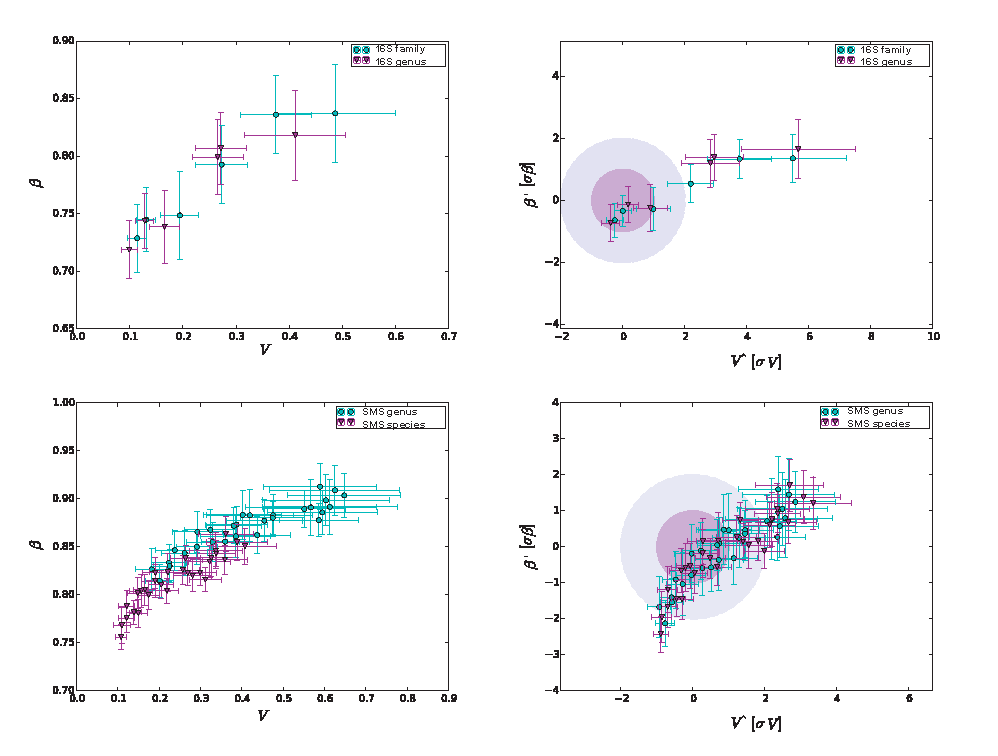
\includegraphics[width=1.0\textwidth]{figs/supfig_taxlev1.eps}
\caption{Overview of the comparison of different approaches based on adjacent taxonomic levels using plots in the Taylor-parameters space. The former row of subfigures is for 16S, where levels are family (blue circles) vs. genus (purple triangles), whereas the latter row of subfigures is for SMS, where levels are genus (blue circles) vs. species (purple triangles). The left column shows the raw results and the right column plots the standardized results (see Standardization in Material and Methods).}
\label{supfig:taxlev1}
\end{supfig}

\begin{supfig} 
  %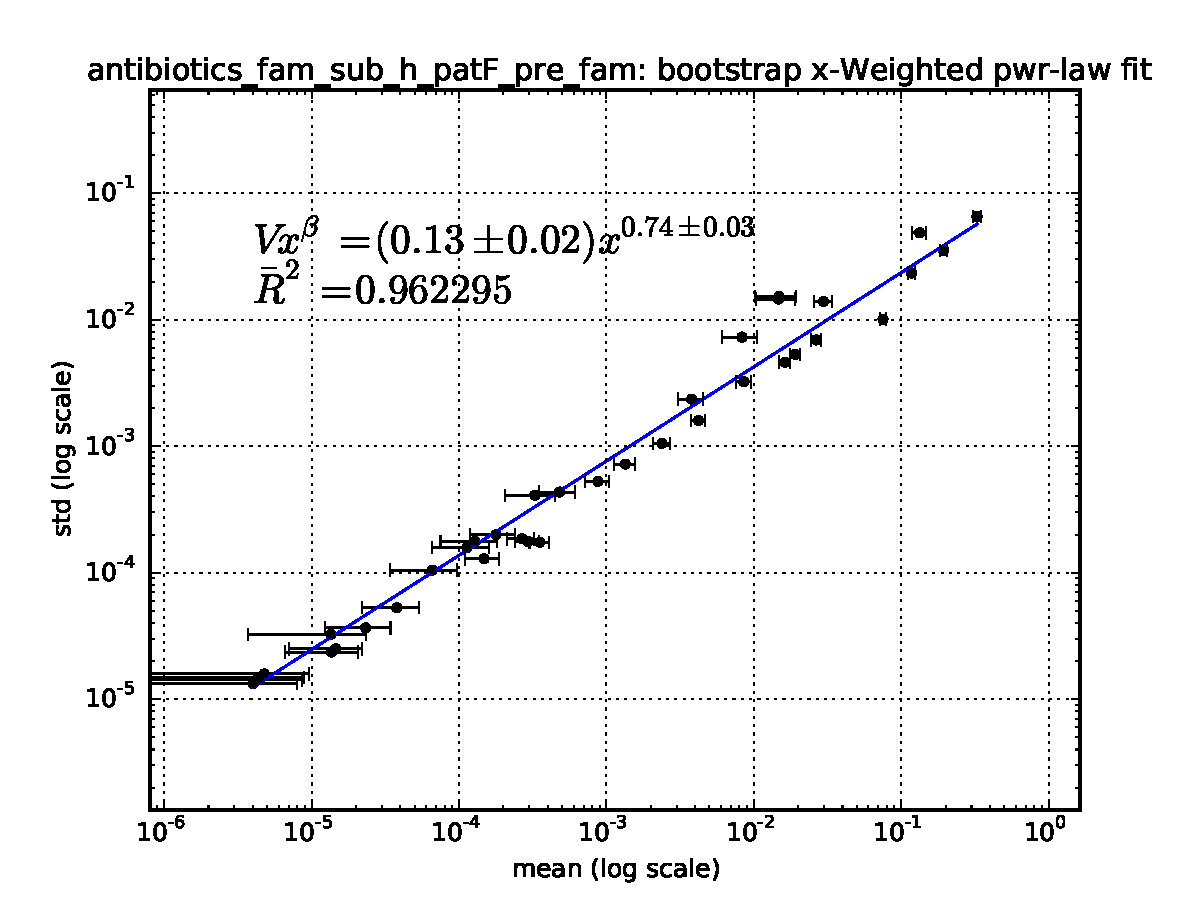
\includegraphics[width=0.5\textwidth]{results/taxalevel/xWb_fam_16S.pdf}
  %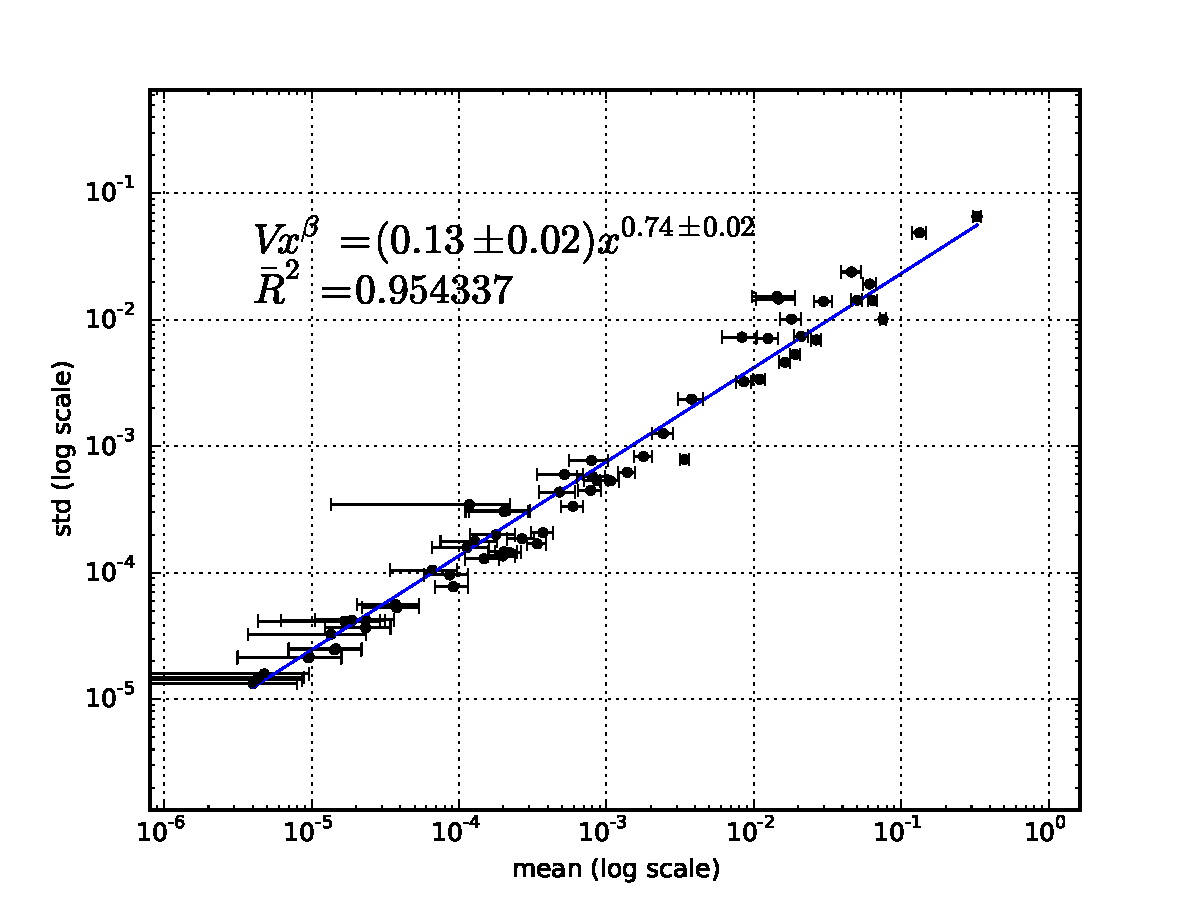
\includegraphics[width=0.5\textwidth]{results/taxalevel/xWb_gen_16S.pdf}
  %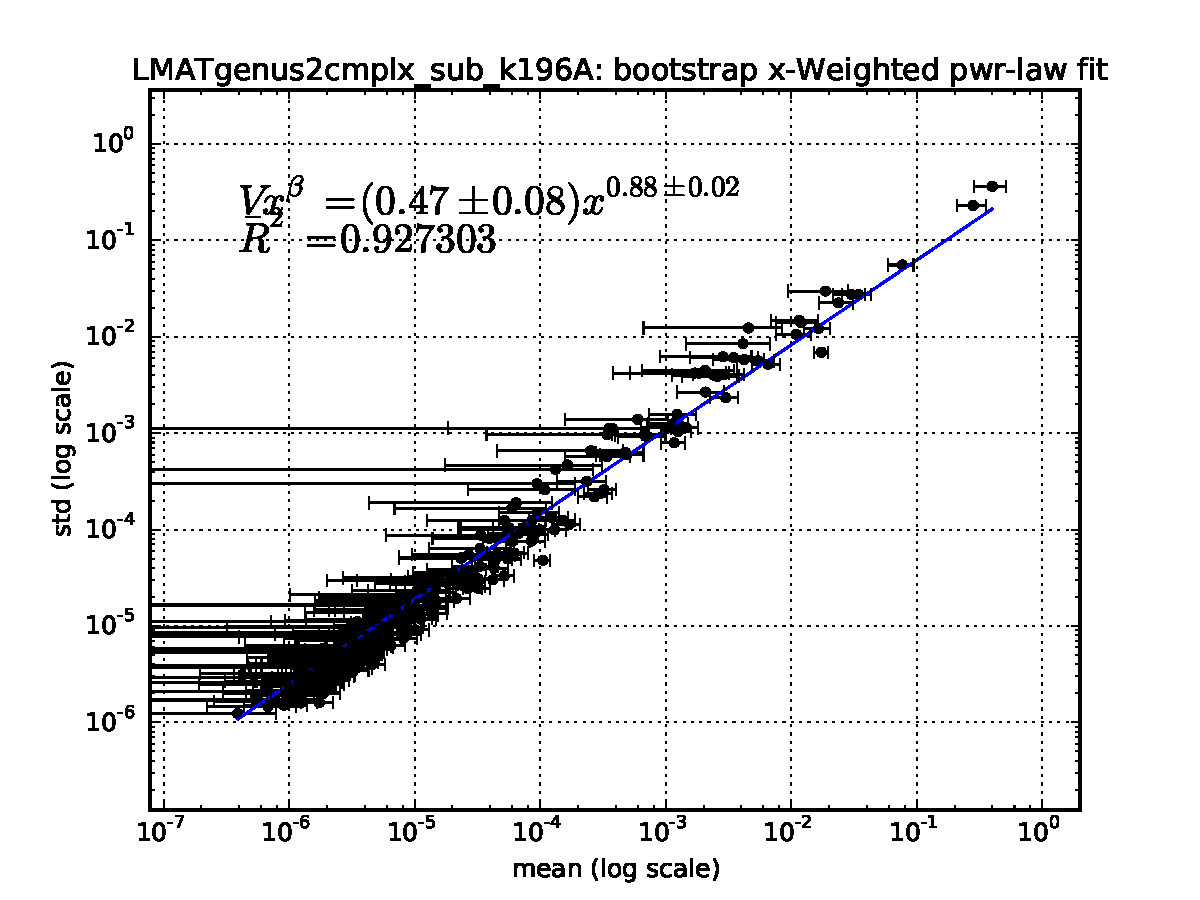
\includegraphics[width=0.5\textwidth]{results/taxalevel/xWb_gen_SMS.pdf}
  %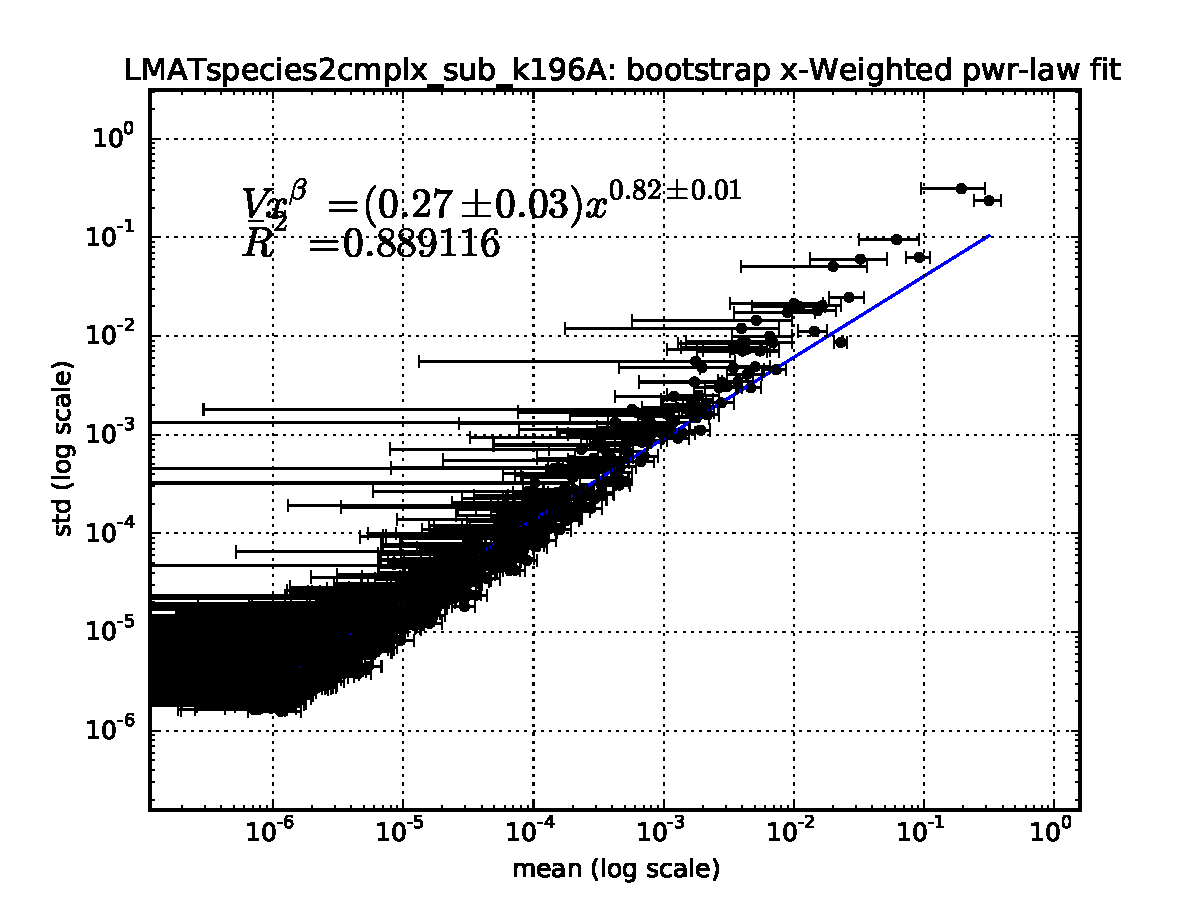
\includegraphics[width=0.5\textwidth]{results/taxalevel/xWb_spc_SMS.pdf}
  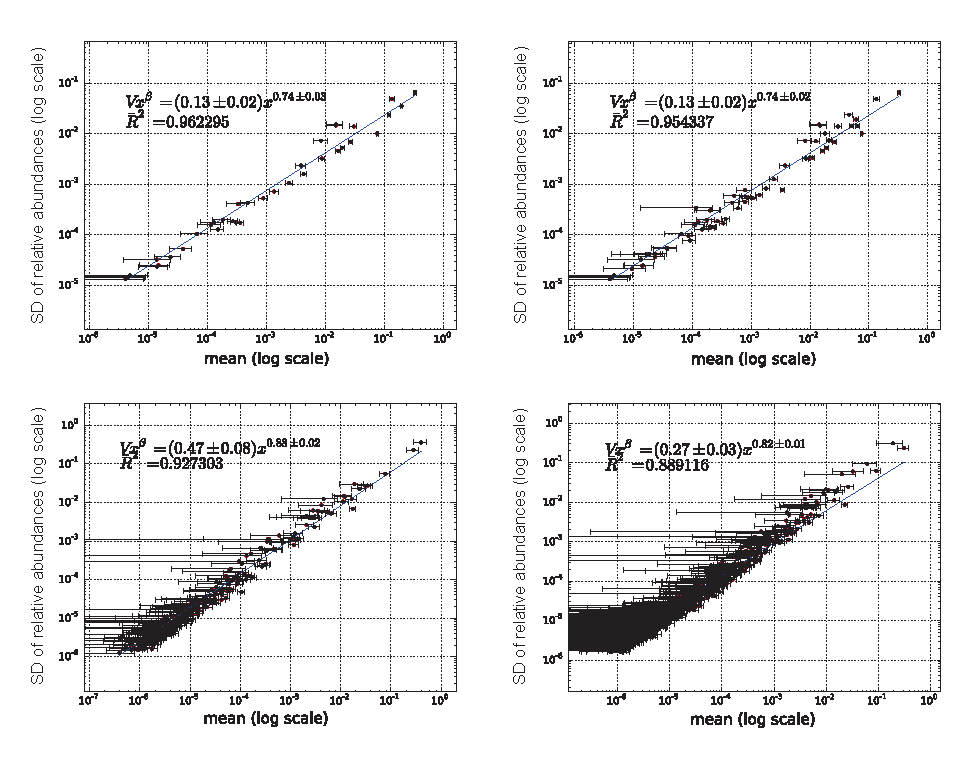
\includegraphics[width=1.0\textwidth]{figs/supfig_taxlev2.eps}
\caption{Detail of comparison of different approaches based on adjacent taxonomic levels using plots of X-weighted power-law fits (see Material and Methods). The former row of subfigures shows examples for 16S, whereas the latter row of subfigures plots examples for SMS. The left column shows results for the superior taxonomic level (family for 16S, genus for SMS), while the right column shows results for the inferior level (genus for 16S, specie for SMS).}
\label{supfig:taxlev2}
\end{supfig}
%TC:ignore

%%
\subsection*{X-weighted power-law fit}\label{sec:X-w}

When fitting the power-law of std vs. mean, we took into account that every mean has uncertainty and can be estimated for a sample size $n$ by the SEM (\emph{Standard Error of the Mean}). Here, the uncertainties affected the independent variable, so the fit was not as trivial as a Y-weighted fit, where the uncertainties affect the dependent variable. A standard approach for this fit is: a) to invert the variables before applying the weights, b) then perform the weighted fit, and finally, c) revert the inversion. This method is deterministic, but the approximate solution worsens with smaller coefficients of determination. To overcome this limitation, we developed a stochastic method by using a bootstrapping-like strategy that avoided inversion and could be applied regardless of the coefficient of determination.

The basic idea of bootstrapping is that inference about a population from sample data (sample $\rightarrow$ population) can be modeled by resampling the sample data and performing inference on (resample $\rightarrow$ sample)\cite{boot}. To adapt this general idea to our problem, we resampled the x-data array using its errors array. That is, for each replicate, a new x-data array was computed based on:
\begin{linenomath}
$$x^*_i = x_i + v_i$$
\end{linenomath}
where $v_i$ is a Gaussian random variable with mean $\mu_i=0$ and standard deviation $\sigma_i=\mathrm{SEM}_i$, as defined previously. For each replicate, a complete unweighted power-law fit was performed, where in order to choose between fitting power laws ($y=Vx^\beta$) using linear regression on log-transformed (LLR) data versus non-linear regression (NLR) we mainly followed the \emph{General Guidelines for the Analysis of Biological Power Laws}\cite{biopwrlaw}. The parameters of the X-weighted fit were then estimated by averaging through all the replicate fits performed, and their errors were estimated by computing the standard deviation for all the fits. At the end of each step, the relative error was calculated by comparing the fit parameter estimation in the last step with the previous one. Finally, both the coefficient of determination of the fit and the coefficient of correlation between the fit parameters were estimated by averaging.

%%
\subsection*{Rank Stability Index}\label{sec:RSI}

The Rank Stability Index (RSI) is shown as a percentage in a separate bar on the right of the rank matrix plot in Figures \ref{fig:corrank_HLS_abroad} and \ref{fig:corrank_HLS_returned} and Supplementary Figures S\ref{supfig:corrank_HLS_before} and S\ref{supfig:corrank_HLS_after}. The RSI is strictly $1$ for an element whose range never changes over time, and is strictly $0$ for an element whose rank oscillates between the extremes over time. So, the RSI is calculated, per element, as $1$ less the quotient of the number of true rank hops taken between the number of maximum possible rank hops, all powered to $p$:
\begin{linenomath}
$${\rm RSI} = \left(1-\frac{\text{true rank hops}}{\text{possible rank hops}}\right)^p = \left(1-\frac{D}{(N-1)(t-1)}\right)^p$$
\end{linenomath}
where $D$ is the total of rank hops taken by the studied element, $N$ is the number of elements that have been ranked, and $t$ is the number of time samples. The power index $p=4$ was arbitrarily chosen to increase the resolution in the stable region.

Finally, under the rank matrix of the aforementioned Figures there are plots relevant to the variability of the rank over time. On the one hand, the RV (Rank Variability) for a sampling point shows the absolute difference between every taxon?s rank and its accumulated abundance rank (the overall rank), averaged for all the taxa shown. On the other hand, the DV (Differences Variability) for a sampling point shows the absolute difference between every taxon?s rank at that time and the value that it had at the previous sampling point, averaged for all the taxa shown.

%\normalsize
%TC:endignore